\chapter{Náhodná veličina a náhodný vektor}
\section{Úplná soustava jevů}
Nechť je dán pravděpodobnostní prostor $\{\Omega,\mathscr{F},P\}$. Soustavu jevů $A_i\in\mathscr{F}$ nazveme \textbf{úplnou soustavou jevů}, jestliže platí $i\neq j$ platí $A_i\cap A_j=\emptyset$ a jestliže jev \uv{nastane jeden z jevů $A_i, i=1,2,\ldots$} nastane s pravděpodobností 1, tj.

\[ P\left(U\bigcup_{i=1}^\infty A_i\right)=\sum_{i=1}^\infty P(A_i)=1 \]

\subsection{Rozdělení pravděpodobností}
Je-li $A_i\in\mathscr{F}$ úplnou soustavou jevů, nazveme pravděpodobnosti $P(A_i)$ \textbf{rozdělením pravděpodobnosti}.

\subsection{Věta o úplné pravděpodobnosti}
Nechť $A_i,i=1,2,\ldots$ je úplná soustava jevů a platí $P(A_i)>0$ pro $i=1,2,\ldots$. Potom pro libovolnou množinu $B\in\mathscr{F}$ platí

\[ P(B)=P(B\cap \Omega)=P(B\cap \left(\bigcup_{i=1}^\infty A_i\right)=P\left( \bigcup_{i=1}^\infty A_i\cap B\right) \]

Protože $A_i$ jsou navzájem disjunktní, jsou disjunktní i průniky $A_i\cap B$. Tudíž lze pravděpodobnost součtu zapsat jako součet pravděpodobností.

\[ P(B) = \sum_{i=1}^\infty P(A_i\cap B)\quad \text{a víme, že } P(B|A_i)=\frac{P(A_i\cap B)}{P(A_i)} \]

Dosazením podmíněné pravděpodobnosti dostáváme větu o úplné pravděpodobnosti ve tvaru

\[ P(B)=\sumi P(B|A_i)P(A_i) \]

\subsection{Bayesova věta}
Platí, že

\[ P(A_i|B)=\frac{P(B|A_i)P(A_i)}{P(B)} \]

je-li $A_i,i=1,2,\ldots$ úplnou soustavou jevů. Pak

\[ P(A_i|B)=\frac{P(B|A_i)P(A_i)}{\displaystyle\sumi[j] P(B|A_j)P(A_j)} \]

\section{Náhodné veličiny}
Transformace základního prostoru, motivace pro specifikaci vhodné transformace: Pravděpodobnostní prostor $\{\Omega, \mathscr{F}, P\}$, množinu $\Gamma$ a zobrazení $X:\Omega\to\Gamma$, které každému prvku $\omega$ přiřazuje právě jeden prvek $\gamma$, kde

\[ \gamma=X(\omega)\in\Gamma \]

Označíme symbolem $B\subset\Gamma$, pak jev $\gamma\in B$ může, ale nemusí být pravděpodobnostním jevem.

\begin{note}{Příklad}
Nechť $\Omega=\{a,b,c\}, F=\{\emptyset,\Omega,a,\{b,c\}\}, P:\mathscr{F}\to\mathbb{R}$. Dále nechť $\Gamma=\{1,2\}$ a zobrazení $X:\Omega\to\Gamma$ definované

	\begin{figure}
		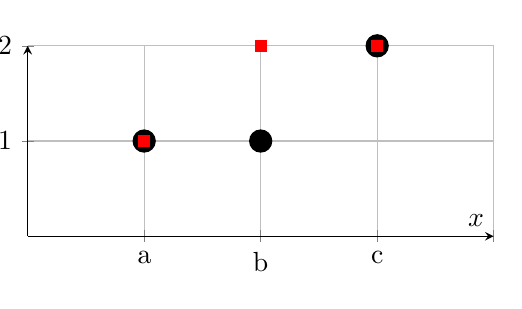
\begin{tikzpicture}[trim axis left, trim axis right]
		\begin{axis}[
		height=4cm,
		width = 7.5cm,
		axis lines=middle,
		xlabel={$x$},
		ylabel={$y$},
		ylabel near ticks,
		ymin=0, ymax=2,
		xmin=0, xmax=4,
		ytick = {0,1,2},
		xtick = {},
		xticklabels = {0,0,a,b,c},
		grid = both
		]
		\addplot [only marks, mark size = 4] table {
		1 1
		2 1
		3 2
		};
		\addplot [only marks, mark=square*, mark size = 2, fill=red, draw=red] table {
		1 1
		2 2
		3 2
		};
	\end{axis}
\end{tikzpicture}
	\end{figure}

	pak jev $\gamma\in\{1\}$ nastává právě tehdy, když $\omega\in\{a,b\}$ ale ten nepatří do $\mathscr{F}$, není jevem pravděpodobnostním, a tedy ani $\gamma$ není jevem pravděpodobnostním. Pokud změníme zobrazení ({\color{red}$\blacksquare$}), pak

	\begin{eqnarray*}
	P(\{1\}) &=& P(\{a\})\\
	P(\{2\}) &=& P(\{a,b\})
	\end{eqnarray*}

	jev $\gamma\in B, B\subset\Gamma$ daná zobrazením $\gamma:X(\omega)$ je pravděpodobnostním jevem právě tehdy, když je pravděpodobnostním jevem jev $X^{^-1}(B)$, tedy jestliže

	\[ X^{-1}(B)\in\mathscr{F} \]

	Označíme-li symbolem $\mathscr{B}$ soubor všech jevů $B\subset\Gamma$, pro které platí $X^{-1}(B)\subset\mathscr{F}$, pak tento soubor tvoří $\sigma$-algebru na množině $\Gamma$, pro jejichž pravděpodobnost $P(B),B\in\mathscr{B}$ platí

	\[ P(B)=P(X^{-1}(B)) \]

	Uspořádaná trojice $(\Gamma,\mathscr{B},P)$ se nazývá \textbf{pravděpodobnostním prostorem}, který je indukovaný původním pravděpodobnostním prostorem $\brs{\Omega,\mathscr{F}, P}$.
	\end{note}

	\section{Obecná náhodná veličina}
	\subsection{Definice náhodné veličiny}
	Pro každé měřitelné zobrazení
	\[ X: (\Omega,\mathscr{F},P)\to(\Gamma,\mathscr{T}), \]

	kde $\Gamma$ je množina a $\mathscr{T}$ je topologie platí $X^{-1}(B)\in\mathscr{F}$, pro každé $B\in\mathscr{B}$, kde topologie $\mathscr{T}$ je definovaná systémem borelovských množin $\mathscr{B}$.\br

	Každý jev z borelovské $\sigma$-algebry $\mathscr{B}$ je pravděpodobnostním jevem s pravděpodobností

	\[ P(B)=P(X^{-1}(B)) \]

	Zobrazení $X:\Omega\to\Gamma$ nazveme \textbf{obecnou náhodnou veličinou}.

	\subsubsection{Speciální případ $\Gamma=\mathbb{R}$}
	Mějme pravděpodobnostní prostor $(\Omega,\mathscr{F},P)$ a topologický prostor reálných čísel s přirozenou topologií $(\mathbb{R},\mathscr{T})$. Potom měřitelné zobrazení $X:\Omega\to\mathbb{R}$ nazveme náhodnou veličinou.

	\subsection{Distribuční funkce náhodné veličiny}
	Je-li $\Gamma=\mathbb{R}$, pak stačí znát pravděpodobnost všech jevů množiny $\mathscr{B}$, které lze vyjádřit například ve tvaru intervalu $(-\infty,a), a\in\mathbb{R}$ (lze i další otevřené a uzavřené intervaly).\br

	Nechť máme pravděpodobnost intervalů $P((-\infty,x))$ pro všechna $x\in\mathbb{R}$, to jest pravděpodobnost všech jevů na $\mathscr{B}$, kterou lze zapsat ve tvaru $(-\infty, x)$, resp. jim odpovídajícím jevů $\brs{\omega: X(\omega)<x}$.

	\[ P((-\infty,x))=P(X^{-1}((-\infty,x))), \]

	kde inverze $X^{-1}=\brs{\omega: X(\omega)<x}$ je jev na $\sigma$-algebře $\mathscr{F}$. Čili pravděpodobnost, že hodnota $X(\omega)$ je menší, než libovolné číslo $x\in\mathbb{R}$ se nazývá \textbf{distribuční funkce} náhodné veličiny $x$ a značí se symbolem $F_X(\cdot)$ a definovaná vztahem

	\[ F_X(x)=P(\brs{\omega:X(\omega)<x}) \]

	\begin{note}{Poznámka}
	Pokud nehrozí záměna, píše se pouze argument $F(x)$.
	\end{note}

	\subsection{Vlastnosti distribuční funkce}
	\begin{itemize}
	\item $F_X(x)$ je \textbf{neklesající funkce} (posouváním $x$ v intervalu $(-\infty,x)$ nám nemůže pravděpodobnost snížit)
	\item $F_X(x)$ je \textbf{zleva spojitá}
	\[ \lim_{h\to 0^+} F_X(x-h)=F_X(x) \]
	\item Limity do nekonečna
	\begin{eqnarray*}
	\lim_{x\to-\infty} F_X(x) & = & 0\\
	\lim_{x\to\infty} F_X(x) & = & 1
	\end{eqnarray*}
	\end{itemize}

	\begin{note}{Poznámka}
	Každá funkce $F_X(x)$, která splňuje výše uvedené vlastnosti, je distribuční funkcí nějaké náhodné proměnné $X$.
	\end{note}

	\subsection{Hustota pravděpodobnosti}
	Pokud existuje funkce $p_X(x)$ definovaná tak, že

	\[ F_X(x) = \int\limits_{-\infty}^x p_x(\xi)\d\xi, \]

	pak $p_X(x)$ se nazývá \textbf{hustota pravděpodobnosti} náhodné veličiny $X$.

	\section{Náhodný vektor}
	N-rozměrnou náhodnou veličinu (náhodný vektor) budeme nazývat n-tici $X=(\vecrow[X])$, jejíž složky $X_i, i=1,2,\ldots$ jsou náhodnými veličinami. Alternativní definice může být za předpokladu, že je $\Gamma=\mathbb{R}^n$.

	\subsection{Distribuční funkce náhodného vektoru}
	Distribuční funkce náhodného n-rozměrného vektoru je funkce n-rozměrného vektoru $x$ definovaná vztahem

	\begin{eqnarray*}
	F_X(x)& = &F_{\vecrow[X]}(\vecrow[X])=\\
	&=&P(\brs{\omega: X_1(\omega)<x_1, X_2(\omega)<x_2,\ldots,X_n(\omega)<x_n})
	\end{eqnarray*}

	\subsection{Vlastnosti distribuční funkce náhodného vektoru}
	\begin{itemize}
	\item $F_X(x)$ je \textbf{neklesající} funkcí každé své proměnné
	\item $F_X(x)$ je \textbf{zleva spojitá} každé své proměnné
	\item $F_{\vecrow[X]}(\vecrow[x])=0$, platí-li alespoň pro jednu $x_i\to-\infty$.
	\item $F_{\vecrow[X]}(\vecrow[x])=1$, platí-li $x_i\to\infty$ pro všechna $i$.
	\item $\lim_{x_n\to\infty}F_{\vecrow[X]}(\vecrow[x])=F_{X_1\ldots X_{n-1}}(x_1\ldots x_{n-1})$
	\item $F_{\vecrow[X]}(\vecrow[x])=F_{X_{z_1},\ldots,X_{z_n}}(x_{z_1},\ldots,x_{z_n})$
	\end{itemize}

	\subsection{Hustota pravděpodobnosti náhodného vektoru}
	Pokud existuje $p_X(\vecrow[x])$ taková, že

	\[ F_X(\vecrow[x])=\int\limits_{-\infty}^{x_1}\int\limits_{-\infty}^{x_2}\cdots\int\limits_{-\infty}^{x_n} p_X(\vecrow[\xi])\vecrow[\d\xi], \]

	pak $p_X(\vecrow[x])$ se nazývá \textbf{hustota pravděpodobnosti}.

	\begin{note}{Poznámka}
	Pokud existuje parciální derivace
	\[ \frac{\partial^n F_X(\vecrow[x])}{\vecrow[\partial x]}, \]

	pak platí
	\[ p_X(\vecrow[x])=\frac{\partial^n F_X(\vecrow[x])}{\vecrow[\partial x]} \]

	Užitečný vztah
	\[ P_{X_1,X_2,\ldots X_{n-1}}(x_1,x_2,\ldots x_{n-1}) = \int\limits_{-\infty}^\infty P_{X_1,X_2,\ldots X_{n-1}}(x_1,x_2,\ldots x_{n-1})\d x_n \]
	\end{note}

	\subsection{Podmíněná distribuční funkce}
	Nechť je dán pravděpodobnostní prostor $(\Omega,\mathbb{F},P)$, nechť $A,B\in\mathscr{F}$, pak pro $P(B)\neq 0$ platí
	\[ P(A|B)=\frac{P(A\cap B)}{P(B)} \]

	Mějme topologický prostor $(\mathbb{R},\mathscr{T})$ (reálná čísla, přirozená topologie) a měřitelné zobrazení $X,Y$ prostoru $(\Omega,\mathscr{F},P)$ do prostoru $(\mathbb{R},\mathscr{T})$.\br

	Vzorem každé borelovské množiny $(\mathbb{R},\mathscr{T})$, jehož $\sigma$-algebru borelovských množin značíme $\mathscr{B}$ je měřitelná množina pravděpodobnostního prostoru $(\Omega,\mathscr{F},P)$. Jsou-li $U,V$ borelovské množiny na $(\mathbb{R},\mathscr{T})$, jsou inverze $X^{-1}(U),Y^{-1}(V)$ měřitelné množiny pravděpodobnostního prostoru $(\Omega,\mathscr{F},P)$. Existují tedy pravděpodobnosti

	\[ P(X^{-1}(U), P(Y^{-1}(V)), P(X^{-1}(U)\cap Y^{-1}(V)) \]

	a podmíněná pravděpodobnost obou inverzí, tedy

	\[ P(X^{-1}(U),Y^{-1}(V)) =\frac{P(X^{-1}(U)\cap Y^{-1}(V))}{P(Y^{-1}(V))}\]

	(pokud $P(Y^{-1}(V))\neq 0$). Podmíněnu pravděpodobností je pravděpodobnost, že hodnota $X(\omega)$ patří do množiny $U$ za podmínky, že $Y(\omega)$ patří do množiny $V$.

	\subsubsection{Podmíněná distribuční funkce}
	Podmíněná pravděpodobnost

	\[ P(X^{-1}((-\infty,x))|Y^{-1}(\brs{y}) \]

	se nazývá \textbf{podmíněná distribuční funkce} náhodné veličiny $X$ za podmínky $Y(\omega)=y$. Značíme

	\[ F_X(x|y)=P(X^{-1}((-\infty,x))|Y^{-1}(\brs{y}) \]

	pro $U=(-\infty,x), V=(-\infty,y)$.

	\[ F_{X,Y}(x,y)=\int_{-\infty}^y F(x|y)\d F(y) \]

	\subsection{Podmíněná distribuční funkce náhodných vektorů}
	Mějme $X$ jako n-rozměrnou náhodnou veličinu a $Y$ jako m-rozměrnou náhodnou veličinu. Pak distribuční funkce náhodného vektoru $X$ za podmínky $Y(\omega)=y$.

	\[ F(\vecrow[x]|\vecrow[y]) = P(X_1(\omega)<x_1,\ldots,X_n(\omega)<x_n | Y_1(\omega)<y_1,\ldots,Y_n(\omega)<y_n) \]

	platí

	\[ F(x_1,\ldots,x_n,y_1,\ldots,y_n) = \int\limits_{-\infty}^{y_n}\cdots\int\limits_{-\infty}^{y_m} F(x_1\ldots,x_n|y_1,\ldots,y_n)\d F(y_1,\ldots,y_n) \]

	\subsection{Podmíněná hustota pravděpodobnosti}
	Existuje-li $P(\svecrow[x]|\svecrow[y])$ taková, že

	\[ F(\svecrow[x],\svecrow[y])=\int\limits_{-\infty}^{x_1}\cdots\int\limits_{-\infty}^{x_n}p(\svecrow[\xi]|\svecrow[y])\svecrow[\d\xi], \]

	pak je to podmíněná hustota pravděpodobnosti.
	\[ P(\svecrow[x],\svecrow[y])=P(\svecrow[x]|\svecrow[y])\cdot P(\svecrow[y]) \]

	vektorově $P(\vec{x},\vec{y})=P(\vec{x},\vec{y})\cdot P(\vec{y})$.